\chapter{Vector Calculus and Differential Geometry of Trajectories}
\label{ch:vectors}

\begin{chapterintro}
\textbf{Chapter Objectives:} In this chapter, we develop the mathematical machinery of vectors and vector fields that governs classical mechanics. You will master the geometry of scalar, vector, and triple products; understand Poisson's kinematic formula for rotating frames; and wield the differential vector operators ($\grad, \divg, \rot$) to determine whether physical force fields are conservative.
\end{chapterintro}

\section{Vector Algebra in Three Dimensions}

Let $\mathcal{E}^3$ be three-dimensional Euclidean space. An orthonormal Cartesian frame is defined by a fixed origin $O$ and an ordered triplet of mutually orthogonal unit vectors $(\ihat, \jhat, \khat)$ satisfying:
\[
\ihat\cdot\ihat = \jhat\cdot\jhat = \khat\cdot\khat = 1, \qquad \ihat\cdot\jhat = \jhat\cdot\khat = \khat\cdot\ihat = 0, \qquad \ihat\times\jhat = \khat.
\]

\begin{figure}[htbp]
\centering
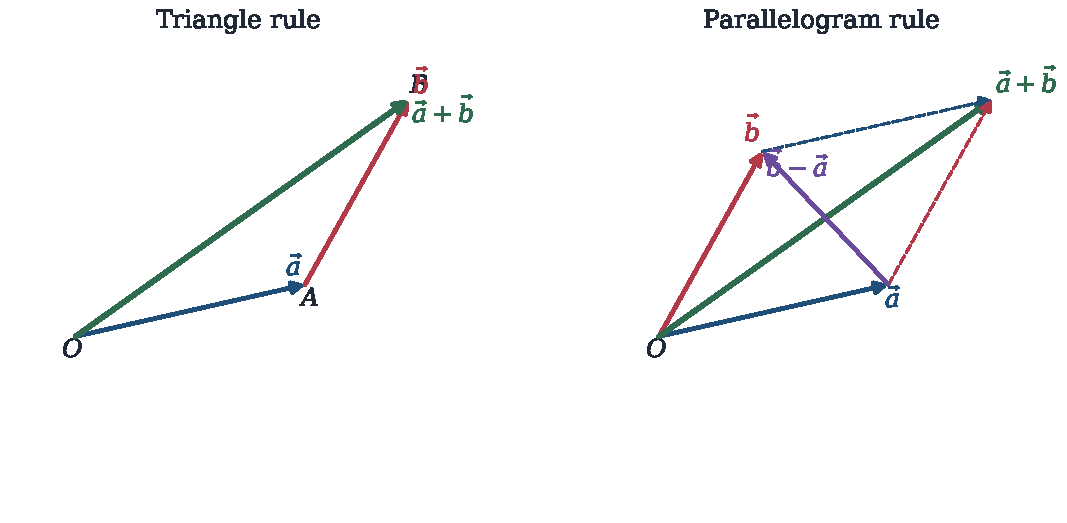
\includegraphics[width=0.74\textwidth]{figures/01_vector_addition.pdf}
\caption{Vector addition and scalar multiplication in Euclidean space. The triangle and parallelogram constructions illustrate $\vec{A} + \vec{B}$.}
\label{fig:vector_addition}
\end{figure}

Any vector $\vec{A}$ can be uniquely resolved into its Cartesian scalar components:
\[
\vec{A} = A_x\,\ihat + A_y\,\jhat + A_z\,\khat.
\]
The Euclidean norm (magnitude) is:
\[
\norm{\vec{A}} = A = \sqrt{\vec{A}\cdot\vec{A}} = \sqrt{A_x^2 + A_y^2 + A_z^2}.
\]

\section{Products of Vectors}

\begin{figure}[htbp]
\centering
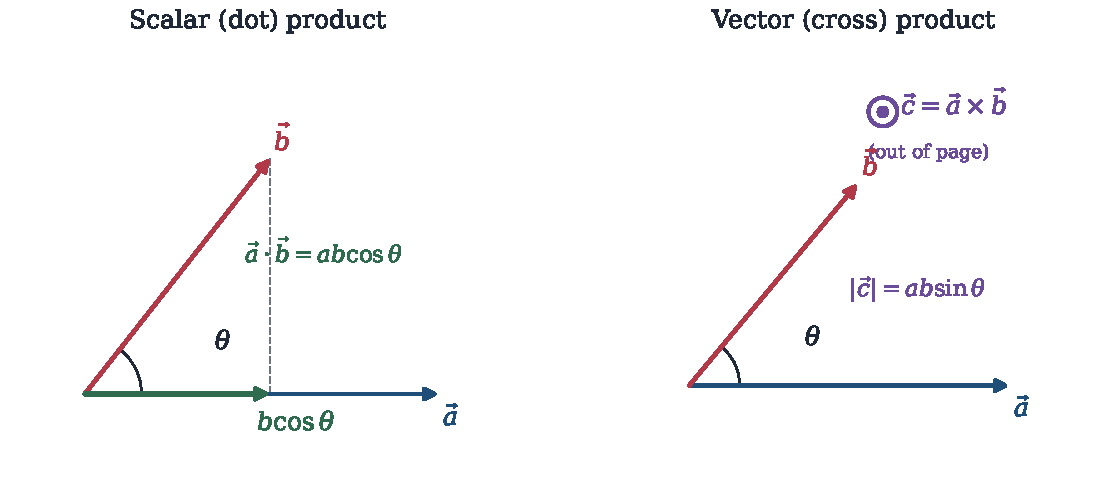
\includegraphics[width=0.78\textwidth]{figures/03_dot_cross.pdf}
\caption{The scalar product $\vec{A}\cdot\vec{B} = AB\cos\theta$ measures collinear projection; the vector product $\vec{A}\times\vec{B}$ yields an orthogonal vector of magnitude $AB\sin\theta$ representing the oriented area of the spanned parallelogram.}
\label{fig:dot_cross}
\end{figure}

\begin{definitionbox}{The Scalar Product (Dot Product)}
The scalar product of two vectors $\vec{A}$ and $\vec{B}$ separated by angle $\theta \in [0, \pi]$ is:
\[
\boxed{\vec{A}\cdot\vec{B} = \norm{\vec{A}}\,\norm{\vec{B}}\cos\theta = A_x B_x + A_y B_y + A_z B_z.}
\]
Two non-zero vectors are orthogonal if and only if $\vec{A}\cdot\vec{B} = 0$.
\end{definitionbox}

\begin{definitionbox}{The Vector Product (Cross Product)}
The vector product $\vec{A}\times\vec{B}$ is a vector orthogonal to both $\vec{A}$ and $\vec{B}$, oriented by the right-hand rule, with magnitude equal to the area of the parallelogram spanned by $\vec{A}$ and $\vec{B}$:
\[
\norm{\vec{A}\times\vec{B}} = \norm{\vec{A}}\,\norm{\vec{B}}\sin\theta.
\]
In Cartesian components, it is expressed as a formal determinant:
\[
\boxed{\vec{A}\times\vec{B} = \begin{vmatrix} \ihat & \jhat & \khat \\ A_x & A_y & A_z \\ B_x & B_y & B_z \end{vmatrix} = (A_y B_z - A_z B_y)\ihat + (A_z B_x - A_x B_z)\jhat + (A_x B_y - A_y B_x)\khat.}
\]
The cross product is anticommutative: $\vec{B}\times\vec{A} = -\vec{A}\times\vec{B}$.
\end{definitionbox}

\begin{lawbox}{The Triple Products and the BAC--CAB Identity}
\begin{itemize}[leftmargin=1.4em,itemsep=3pt]
  \item \textbf{Scalar Triple Product}: $\vec{A}\cdot(\vec{B}\times\vec{c}) = \det[\vec{A}, \vec{B}, \vec{C}]$ represents the oriented volume of the parallelepiped spanned by the three vectors. It is invariant under cyclic permutations:
        \[
        \vec{A}\cdot(\vec{B}\times\vec{C}) = \vec{B}\cdot(\vec{C}\times\vec{A}) = \vec{C}\cdot(\vec{A}\times\vec{B}).
        \]
  \item \textbf{Vector Triple Product (BAC--CAB Rule)}:
        \[
        \boxed{\vec{A}\times(\vec{B}\times\vec{C}) = (\vec{A}\cdot\vec{C})\vec{B} - (\vec{A}\cdot\vec{B})\vec{C}.}
        \]
\end{itemize}
\end{lawbox}

\section{Vector Functions of Time and Poisson's Formula}

When a vector $\vec{A}(t)$ varies with time, its derivative is defined by the standard limit:
\[
\frac{\dd\vec{A}}{\dd t} = \lim_{\Delta t \to 0} \frac{\vec{A}(t + \Delta t) - \vec{A}(t)}{\Delta t} = \dot{A}_x\,\ihat + \dot{A}_y\,\jhat + \dot{A}_z\,\khat.
\]
Differentiating products yields Leibniz rules:
\begin{align*}
\frac{\dd}{\dd t}(\phi\vec{A}) &= \dot{\phi}\vec{A} + \phi\dot{\vec{A}}, \\
\frac{\dd}{\dd t}(\vec{A}\cdot\vec{B}) &= \dot{\vec{A}}\cdot\vec{B} + \vec{A}\cdot\dot{\vec{B}}, \\
\frac{\dd}{\dd t}(\vec{A}\times\vec{B}) &= \dot{\vec{A}}\times\vec{B} + \vec{A}\times\dot{\vec{B}} \quad \text{(order preserved!).}
\end{align*}

\begin{lawbox}{Poisson's Kinematic Formula for Rotating Vectors}
Let $\vec{u}(t)$ be a unit vector of constant length ($\norm{\vec{u}(t)} \equiv 1$).
Then $\vec{u}\cdot\vec{u} = 1$. Differentiating with respect to time:
\[
\frac{\dd}{\dd t}(\vec{u}\cdot\vec{u}) = 2\vec{u}\cdot\frac{\dd\vec{u}}{\dd t} = 0 \implies \frac{\dd\vec{u}}{\dd t} \perp \vec{u}.
\]
Every derivative of a constant-length vector is strictly orthogonal to the vector itself!
Consequently, for any rotating rigid frame with angular velocity vector $\vec{\Omega}$, the rate of change of any vector $\vec{A}$ attached to that frame satisfies:
\[
\boxed{\frac{\dd\vec{A}}{\dd t} = \vec{\Omega}\times\vec{A}.}
\]
\end{lawbox}

\section{Differential Operators in Physics}

In field theories of mechanics, forces are functions of position $\vec{r}$. We define the formal vector differential operator \textbf{del} (nabla):
\[
\vec{\nabla} \equiv \frac{\partial}{\partial x}\ihat + \frac{\partial}{\partial y}\jhat + \frac{\partial}{\partial z}\khat.
\]

\begin{definitionbox}{Gradient, Divergence, and Curl}
\begin{itemize}[leftmargin=1.4em,itemsep=3pt]
  \item \textbf{Gradient} of a scalar field $f(x, y, z)$:
        \[
        \grad f = \vec{\nabla} f = \frac{\partial f}{\partial x}\ihat + \frac{\partial f}{\partial y}\jhat + \frac{\partial f}{\partial z}\khat.
        \]
        $\vec{\nabla} f$ points in the direction of steepest spatial increase of $f$, and its magnitude is the directional derivative in that direction.
  \item \textbf{Divergence} of a vector field $\vec{V}(x, y, z)$:
        \[
        \divg \vec{V} = \vec{\nabla}\cdot\vec{V} = \frac{\partial V_x}{\partial x} + \frac{\partial V_y}{\partial y} + \frac{\partial V_z}{\partial z}.
        \]
        $\vec{\nabla}\cdot\vec{V}$ measures the net flux of $\vec{V}$ emanating per unit volume from a point (sources and sinks).
  \item \textbf{Curl (Rotationnel)} of a vector field $\vec{V}(x, y, z)$:
        \[
        \rot \vec{V} = \vec{\nabla}\times\vec{V} = \begin{vmatrix} \ihat & \jhat & \khat \\ \partial/\partial x & \partial/\partial y & \partial/\partial z \\ V_x & V_y & V_z \end{vmatrix}.
        \]
        $\vec{\nabla}\times\vec{V}$ measures the microscopic circulation or vortex density of the vector field.
\end{itemize}
\end{definitionbox}

\begin{lawbox}{The Irrotational Gradient Identity}
For any twice continuously differentiable scalar function $f(x, y, z)$:
\[
\boxed{\vec{\nabla}\times(\vec{\nabla} f) = \vzero.}
\]
\textbf{Physical Meaning:} Every gradient field is automatically curl-free (irrotational).
Conversely, by Poincaré's Lemma, if a force field $\vec{F}$ is curl-free in a simply-connected domain ($\vec{\nabla}\times\vec{F} = \vzero$), then there exists a potential energy function $E_p(\vec{r})$ such that $\vec{F} = -\vec{\nabla} E_p$.
\end{lawbox}

\section{Extensive Worked Examples}

\begin{workedexample}{The BAC--CAB Expansion and Jacobi Identity}
(a) Prove the BAC--CAB identity $\vec{A}\times(\vec{B}\times\vec{C}) = (\vec{A}\cdot\vec{C})\vec{B} - (\vec{A}\cdot\vec{B})\vec{C}$.
(b) Deduce the \textbf{Jacobi Identity} for the cross product:
\[
\vec{A}\times(\vec{B}\times\vec{C}) + \vec{B}\times(\vec{C}\times\vec{A}) + \vec{C}\times(\vec{A}\times\vec{B}) = \vzero.
\]

\paragraph{Solution.}

(a) Without loss of generality, choose Cartesian coordinates such that $\vec{B}$ lies along the $x$-axis: $\vec{B} = B_x\ihat$, and $\vec{C}$ lies in the $xy$-plane: $\vec{C} = C_x\ihat + C_y\jhat$.
Let $\vec{A} = A_x\ihat + A_y\jhat + A_z\khat$.
The inner cross product is:
\[
\vec{B}\times\vec{C} = (B_x\ihat)\times(C_x\ihat + C_y\jhat) = B_x C_y(\ihat\times\jhat) = B_x C_y\,\khat.
\]
Now compute $\vec{A}\times(\vec{B}\times\vec{C})$:
\begin{align*}
\vec{A}\times(B_x C_y\,\khat) &= (A_x\ihat + A_y\jhat + A_z\khat)\times(B_x C_y\,\khat) \\
&= A_x B_x C_y(\ihat\times\khat) + A_y B_x C_y(\jhat\times\khat) \\
&= -A_x B_x C_y\,\jhat + A_y B_x C_y\,\ihat.
\end{align*}
Now compute the right-hand side $(\vec{A}\cdot\vec{C})\vec{B} - (\vec{A}\cdot\vec{B})\vec{C}$:
\begin{align*}
\vec{A}\cdot\vec{C} &= A_x C_x + A_y C_y, \\
\vec{A}\cdot\vec{B} &= A_x B_x.
\end{align*}
Thus:
\begin{align*}
(\vec{A}\cdot\vec{C})\vec{B} - (\vec{A}\cdot\vec{B})\vec{C} &= (A_x C_x + A_y C_y)(B_x\ihat) - (A_x B_x)(C_x\ihat + C_y\jhat) \\
&= A_x B_x C_x\ihat + A_y B_x C_y\ihat - A_x B_x C_x\ihat - A_x B_x C_y\jhat \\
&= A_y B_x C_y\ihat - A_x B_x C_y\jhat.
\end{align*}
Both expressions are identical! Since the statement is coordinate-independent, the BAC--CAB rule is proven in full generality.

(b) Applying the BAC--CAB rule cyclically to all three permutations:
\begin{align*}
\vec{A}\times(\vec{B}\times\vec{C}) &= (\vec{A}\cdot\vec{C})\vec{B} - (\vec{A}\cdot\vec{B})\vec{C}, \\
\vec{B}\times(\vec{C}\times\vec{A}) &= (\vec{B}\cdot\vec{A})\vec{C} - (\vec{B}\cdot\vec{C})\vec{A}, \\
\vec{C}\times(\vec{A}\times\vec{B}) &= (\vec{C}\cdot\vec{B})\vec{A} - (\vec{C}\cdot\vec{A})\vec{B}.
\end{align*}
Adding all three equations:
Since the dot product is symmetric ($\vec{A}\cdot\vec{C} = \vec{C}\cdot\vec{A}$, $\vec{A}\cdot\vec{B} = \vec{B}\cdot\vec{A}$, $\vec{B}\cdot\vec{C} = \vec{C}\cdot\vec{B}$), every positive term cancels with an identical negative term:
\[
\boxed{\vec{A}\times(\vec{B}\times\vec{C}) + \vec{B}\times(\vec{C}\times\vec{A}) + \vec{C}\times(\vec{A}\times\vec{B}) = \vzero.}
\]
This Jacobi identity confirms that the 3D cross product forms a formal Lie algebra $\mathfrak{so}(3)$ isomorphic to the group of physical rotations!
\end{workedexample}

\begin{workedexample}{Gradient and Curl of Central Force Fields}
Let $\vec{r} = x\ihat + y\jhat + z\khat$ be the position vector, with magnitude $r = \norm{\vec{r}} = \sqrt{x^2 + y^2 + z^2}$, and unit vector $\ur = \vec{r}/r$.
(a) Show that $\vec{\nabla} r = \ur$.
(b) Show that $\vec{\nabla} f(r) = f'(r)\ur$.
(c) Show that any central force field $\vec{F}(\vec{r}) = f(r)\ur$ is irrotational: $\vec{\nabla}\times\vec{F} = \vzero$.
(d) Find the potential energy $E_p(r)$ for Newton's gravitational force $\vec{F}(\vec{r}) = -\frac{GMm}{r^2}\ur$.

\paragraph{Solution.}

(a) Compute the partial derivatives of $r = \sqrt{x^2 + y^2 + z^2}$:
\[
\frac{\partial r}{\partial x} = \frac{2x}{2\sqrt{x^2 + y^2 + z^2}} = \frac{x}{r}, \quad \frac{\partial r}{\partial y} = \frac{y}{r}, \quad \frac{\partial r}{\partial z} = \frac{z}{r}.
\]
Therefore:
\[
\vec{\nabla} r = \frac{\partial r}{\partial x}\ihat + \frac{\partial r}{\partial y}\jhat + \frac{\partial r}{\partial z}\khat = \frac{x}{r}\ihat + \frac{y}{r}\jhat + \frac{z}{r}\khat = \frac{\vec{r}}{r} = \boxed{\ur.}
\]

(b) Applying the chain rule to an arbitrary scalar function $f(r)$:
\[
\frac{\partial f}{\partial x} = \frac{\dd f}{\dd r}\frac{\partial r}{\partial x} = f'(r)\frac{x}{r}.
\]
Assembling the gradient:
\[
\vec{\nabla} f(r) = f'(r)\left(\frac{x}{r}\ihat + \frac{y}{r}\jhat + \frac{z}{r}\khat\right) = \boxed{f'(r)\,\ur.}
\]

(c) We compute the curl of $\vec{F} = f(r)\ur = \frac{f(r)}{r}\vec{r}$.
Using the vector identity $\vec{\nabla}\times(\phi\vec{A}) = \phi(\vec{\nabla}\times\vec{A}) + (\vec{\nabla}\phi)\times\vec{A}$ with $\phi = \frac{f(r)}{r}$ and $\vec{A} = \vec{r}$:
First, compute $\vec{\nabla}\times\vec{r}$:
\[
\vec{\nabla}\times\vec{r} = \begin{vmatrix} \ihat & \jhat & \khat \\ \partial/\partial x & \partial/\partial y & \partial/\partial z \\ x & y & z \end{vmatrix} = (0 - 0)\ihat + (0 - 0)\jhat + (0 - 0)\khat = \vzero.
\]
Second, compute the gradient of the scalar factor $\phi(r)$:
\[
\vec{\nabla}\phi(r) = \phi'(r)\ur.
\]
Now substitute into the identity:
\[
\vec{\nabla}\times\left( \frac{f(r)}{r}\vec{r} \right) = \frac{f(r)}{r}(\vzero) + \left( \phi'(r)\ur \right)\times\vec{r} = \phi'(r)(\ur\times\vec{r}).
\]
Since $\vec{r} = r\ur$, the cross product is:
\[
\ur\times\vec{r} = r(\ur\times\ur) = \vzero.
\]
Therefore:
\[
\boxed{\vec{\nabla}\times\vec{F} = \vzero.}
\]
Every central force field is strictly \textbf{curl-free (conservative)}!

(d) For Newton's gravitational force:
\[
\vec{F}(r) = -\frac{GMm}{r^2}\ur.
\]
Since $\vec{F} = -\vec{\nabla} E_p = -E_p'(r)\ur$:
\[
-E_p'(r) = -\frac{GMm}{r^2} \implies E_p'(r) = \frac{GMm}{r^2}.
\]
Integrating with standard reference at infinity ($E_p(\infty) = 0$):
\[
E_p(r) = -\int_\infty^r \frac{GMm}{r'^2}\dd r' = -\left[ -\frac{GMm}{r'} \right]_\infty^r = \boxed{-\frac{GMm}{r}.}
\]
\end{workedexample}
